Po přihlášení se voliči zobrazí seznam jemu dostupných voleb. Kritéria pro zobrazení voleb: volby jsou aktivní, volič se nachází na seznamu oprávněných voličů. Pokud žádné volby nevyhovují kritériím, je zobrazena informace, že žádné volby nejsou dostupné. Volby se mohou nacházet ve třech stavech: 
\begin{itemize}
	\item Nadcházející - modré orámování, neaktivní desaturované tlačítko \scalebox{.7}[1.0]{\textsf{CAST MY VOTE}}.
	\item Probíhající - Modré orámování, aktivní saturované tlačtíko \scalebox{.7}[1.0]{\textsf{CAST MY VOTE}}.
	\item Ukončené - šedé orámování, saturované tlačítko \scalebox{.7}[1.0]{\textsf{RESULTS}}.
\end{itemize}
\begin{figure}[h]
	\centering
	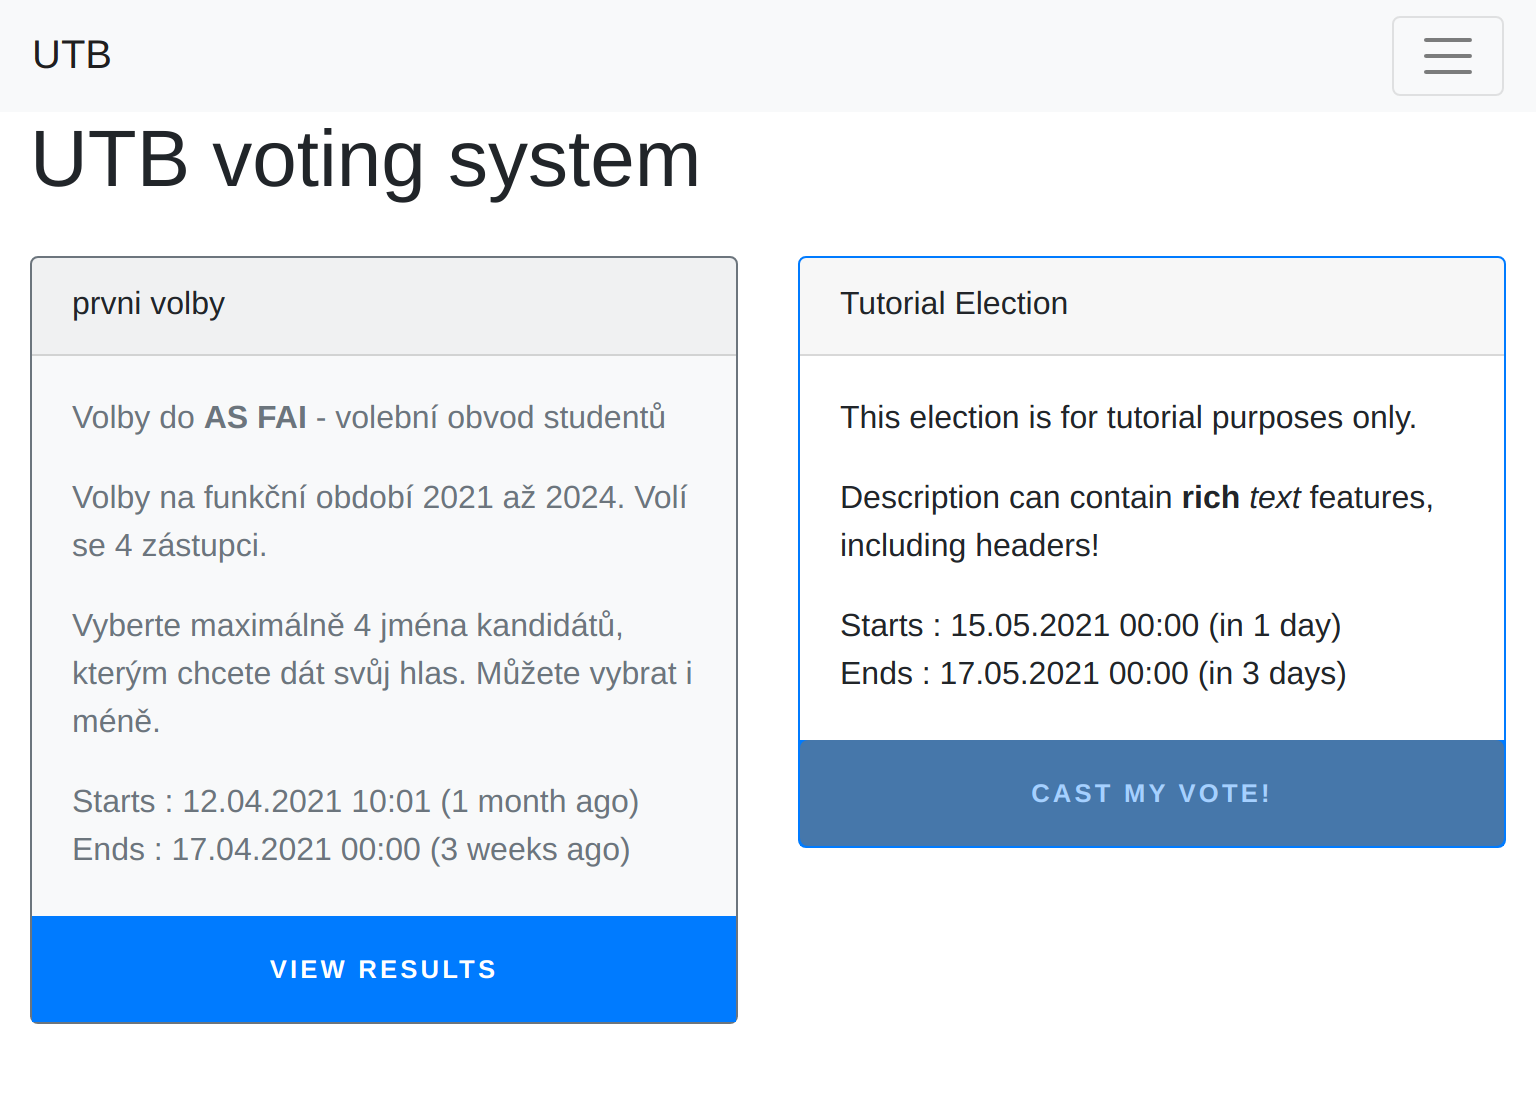
\includegraphics[width=\linewidth]{graphics/attachements/volbyPrehledDouble.png}
	\captionsetup{width=\linewidth}
	\caption*{Obrázek IV.1 Seznam voleb (zdroj: vlastní)}
\end{figure}
\clearpage
Po kliknutí na box s volbami je uživatel přesměrován na stránku hlasování (probíhající volby) nebo výsledků (ukončené volby). Pokud volič již hlasoval a klikne na stejné volby znovu, je přesměrován zpět a infromován chybovou zprávou.

Na stránce s hlasováním může volič zaškrtnout jednotlivé možnosti pro nabízené otázky. Každá otázka je v samostatném boxu a odpovědi řazeny abecedně. Po kliknutí na tlačítko ,,Encrypt the vote'' je provedena validace formuláře. Pokud jsou některé otázky zodpovězeny neplatně, je odesílaní formuláře ukončeno a uživatel o chybách informován zprávou a chyby jsou vyznačeny ve formuláři.

\begin{figure}[h]
	\centering
	\includegraphics[width=\linewidth]{graphics/attachements/volbyCompared.png}
	\captionsetup{width=\linewidth}
	\caption*{Obrázek IV.2 Volební formulář (zdroj: vlastní)}
\end{figure}
\clearpage
Proces šifrování a podepisování hlasovacího lístku probíhá na pozadí bez nutnosti uživatele jakkoli zasahovat. Po dobu kdy aplikace pracuje je zobrazeno dialogové okno s indikátorem čekání. Toto dialogové okno nelze zavřít. 

Po úspěšném odeslání hlasovacího lístku na server je zobrazeno nové dialogové okno, uživatel si může nechat zobrazit podrobnosti šifrování včetně všech šifrovaných dat nebo okno zavřít. Šifrovaná data si může uživatel uschovat pro případný protest. Po zavření kteréhokoli z těchto dvou oken je uživatel přesměrován zpět na domovskou stránku aplikace. 

Původní tlačítko odeslání formuláře je zablokované v momentě kdy je na něj poprvé kliknuto, na serveru je i tak ještě jednou provedena kontrola těsně před uložením lístku, že uživatel ještě v daných volbách nehlasoval.

\begin{figure}[h]
	\centering
	\includegraphics[width=\linewidth]{graphics/attachements/volbyCompared2.png}
	\captionsetup{width=\linewidth}
	\caption*{Obrázek IV.3 Dialogová okna (zdroj: vlastní)}
\end{figure}

\begin{figure}[h]
	\centering
	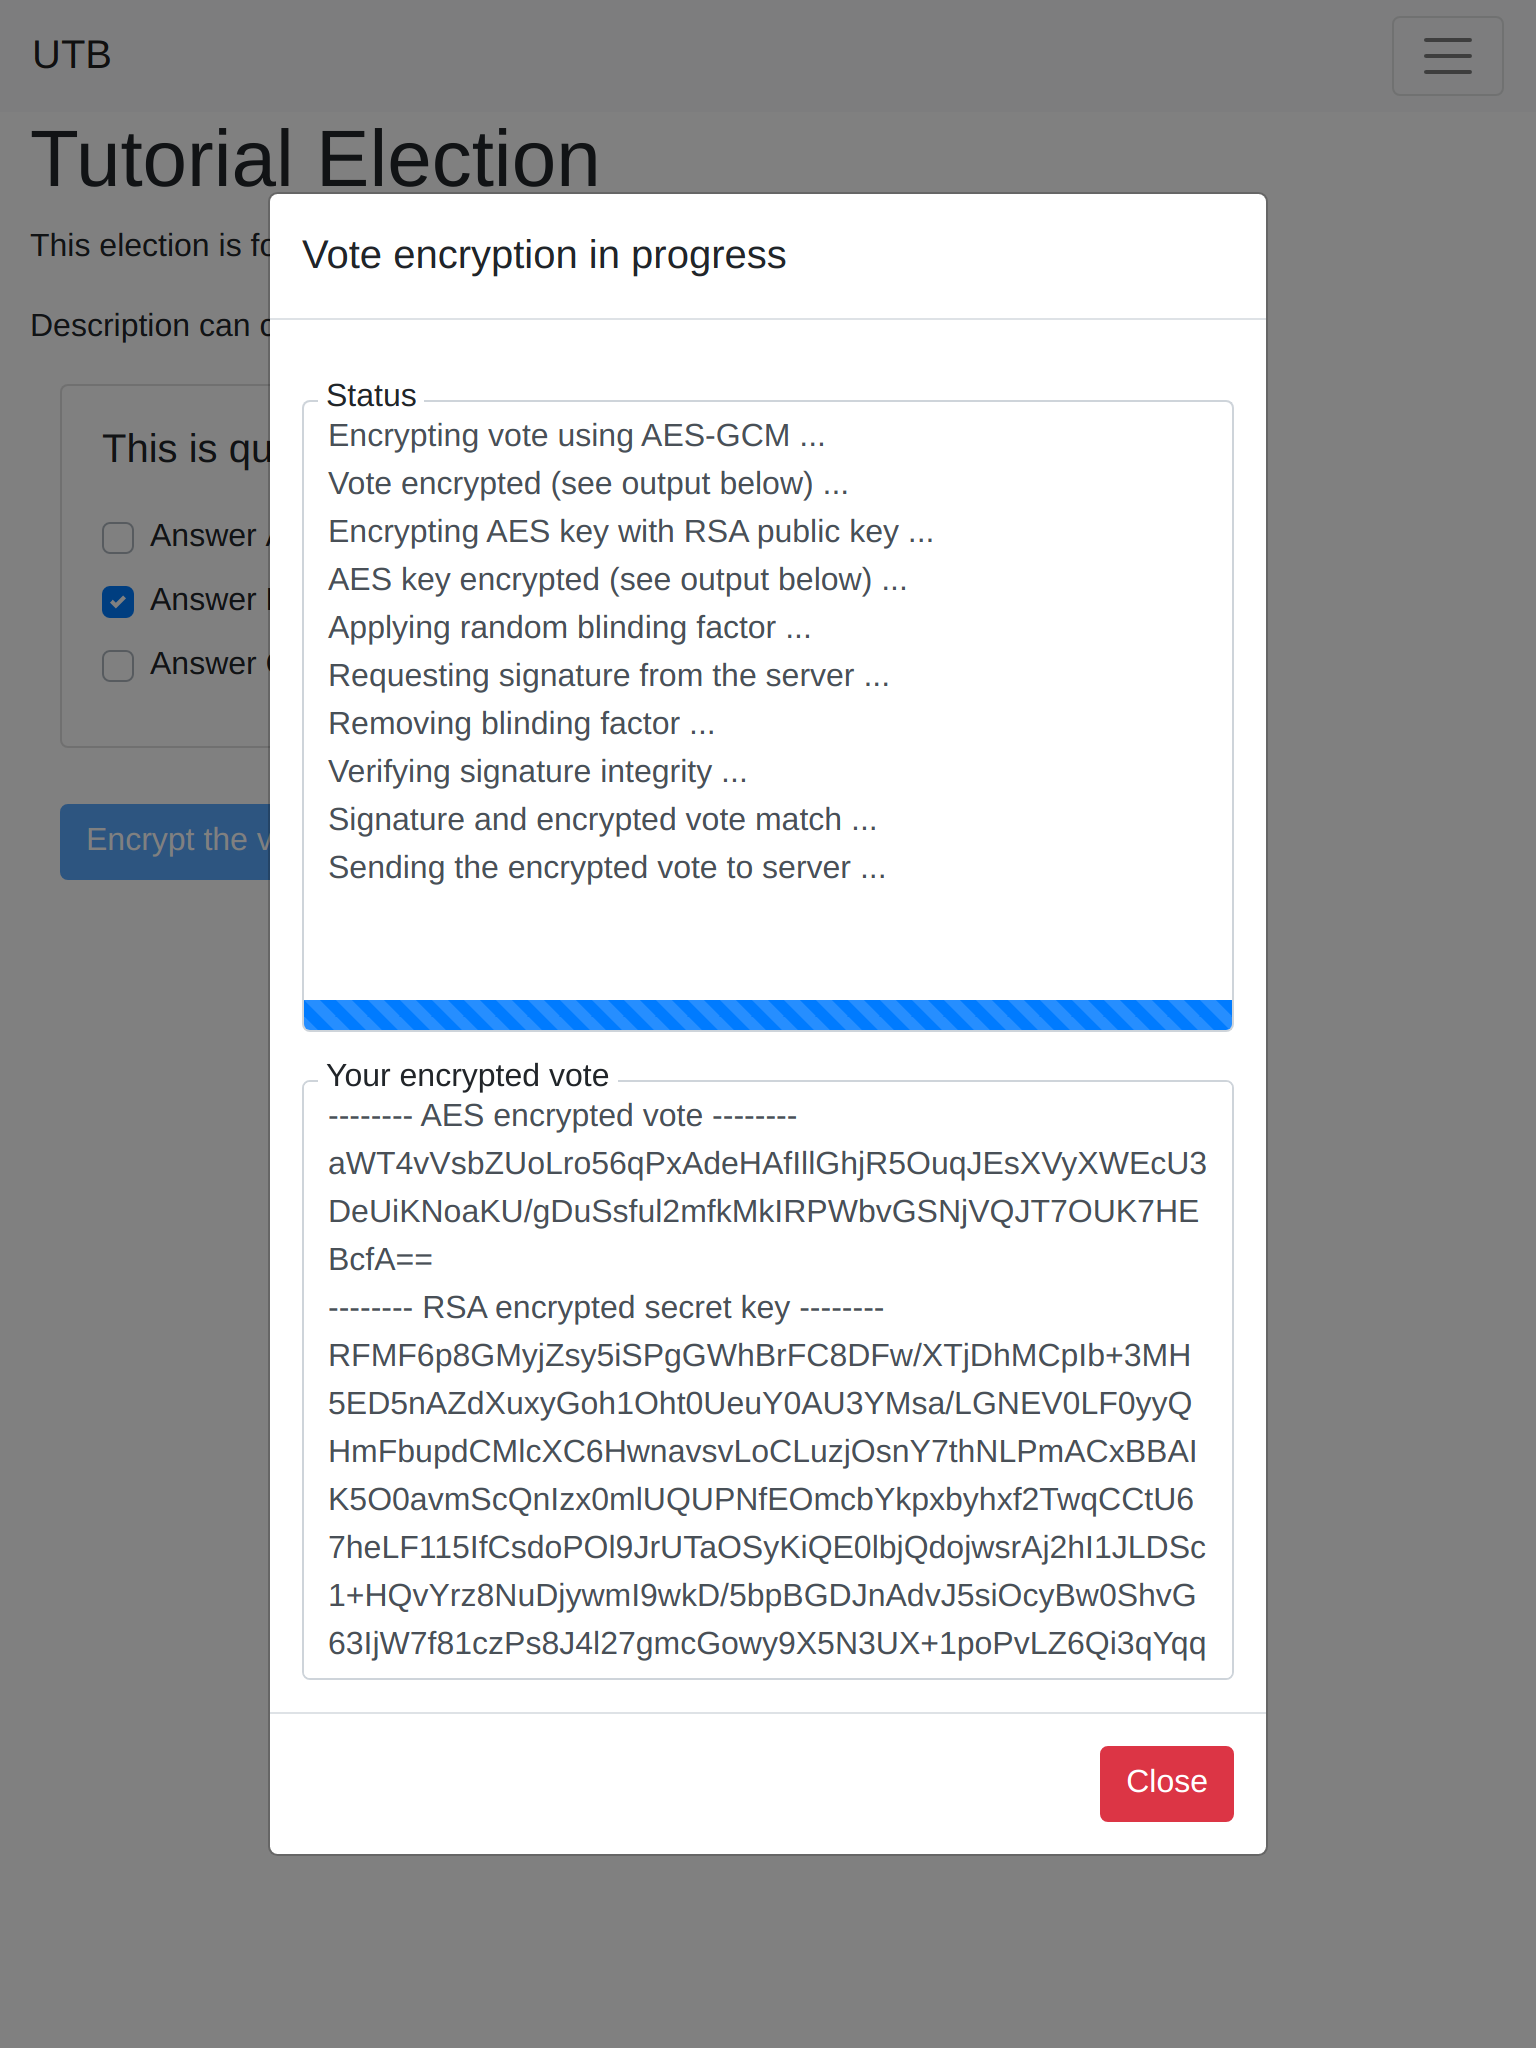
\includegraphics[width=\linewidth]{graphics/attachements/volbyDetails.png}
	\captionsetup{width=\linewidth}
	\caption*{Obrázek IV.4 Detaily šifrovací operace (zdroj: vlastní)}
\end{figure}